%%%%%%%%%%%%%%%%%%%%%%%%%%%%%%%%%%%%%%%%%%%%%%%%%%%%%%%%%%%%%%%%%%%%%%%%%%%%%%%%
% AMS Beamer series / Bologna FC / Template
% Andrea Omicini
% Alma Mater Studiorum - Università di Bologna
% mailto:andrea.omicini@unibo.it
%%%%%%%%%%%%%%%%%%%%%%%%%%%%%%%%%%%%%%%%%%%%%%%%%%%%%%%%%%%%%%%%%%%%%%%%%%%%%%%%
%\documentclass[handout]{beamer}\mode<handout>{\usetheme{default}}
%
\documentclass[presentation, 8pt]{beamer}\mode<presentation>{\usetheme{AMSBolognaFC}}
%\documentclass[handout]{beamer}\mode<handout>{\usetheme{AMSBolognaFC}}
%%%%%%%%%%%%%%%%%%%%%%%%%%%%%%%%%%%%%%%%%%%%%%%%%%%%%%%%%%%%%%%%%%%%%%%%%%%%%%%%
\usepackage[T1]{fontenc}
\usepackage{wasysym}
\usepackage{amsmath,blkarray}
\usepackage[minted,most]{tcolorbox}
\usepackage{centernot}
\usepackage{fontawesome}
\usepackage{fancyvrb}
\usepackage{minted}
\usepackage{hyperref}
\usepackage{multicol}
\setminted[scala]{fontsize=\scriptsize,baselinestretch=1,obeytabs=true, tabsize=2}
\usepackage[ddmmyyyy]{datetime}
\setminted{fontsize=\footnotesize}
\renewcommand{\dateseparator}{}
%\renewcommand{\thefootnote}{\fnsymbol{footnote}}
\newcommand{\version}{1}
\usepackage[
	backend=biber,
	citestyle=authoryear-icomp,
	maxcitenames=1,
	bibstyle=numeric]{biblatex}

	\makeatletter

\addbibresource{biblio.bib}
%%%%%%%%%%%%%%%%%%%%%%%%%%%%%%%%%%%%%%%%%%%%%%%%%%%%%%%%%%%%%%%%%%%%%%%%%%%%%%%%
\title[Programming with ScaFi!]
{Programming (and Learning) Self-Adaptive \& Self-Organising Behaviour with ScaFi}
\subtitle{for Swarms, Edge-Cloud Ecosystems, and More}
%
%
\author[\sspeaker{Casedei}]
{\speaker{Roberto Casadei} \href{mailto:roby.casadei@unibo.it}{roby.casadei@unibo.it} \\
\speaker{Gianluca Aguzzi} \href{mailto:gianluca.aguzzi@unibo.it}{gianluca.aguzzi@unibo.it} \\
\speaker{Danilo Pianini} \href{mailto:danilo.pianini@unibo.it}{danilo.pianini@unibo.it} \\
\speaker{Mirko Viroli} \href{mailto:mirko.viroli@unibo.it}{mirko.viroli@unibo.it}}
%
\institute[DISI, Univ.\ Bologna]
{%Dipartimento di Informatica -- Scienza e Ingegneria (DISI)\\
\textsc{Alma Mater Studiorum} -- Universit{\`a} di Bologna \\[0.1cm]
\textbf{Talk @} \bold{International Conference on Autonomic Computing and Self-Organizing Systems (ACSOS)}}
%
\renewcommand{\dateseparator}{/}
\date[\today]{\today}
%
\AtBeginSubsection[]
{
  \begin{frame}
  \frametitle{Contents}
  \tableofcontents[currentsubsection, 
	sectionstyle=show/shaded, 
	subsectionstyle=show/shaded]
  \end{frame}
}
%%%%%%%%%%%%%%%%%%%%%%%%%%%%%%%%%%%%%%%%%%%%%%%%%%%%%%%%%%%%%%%%%%%%%%%%%%%%%%%%
\begin{document}
%%%%%%%%%%%%%%%%%%%%%%%%%%%%%%%%%%%%%%%%%%%%%%%%%%%%%%%%%%%%%%%%%%%%%%%%%%%%%%%%
\frame{\titlepage}
%===============================================================================
\section{Introduction}
\subsection{Context -- Collective Adaptive Systems}
\begin{frame}{Context}

\end{frame}
\begin{frame}[plain,c]
	\begin{center}
	\Huge \textbf{Collective Adaptive Systems} (CASs)\\
	{\large Systems composed of \emph{possibly} \bold{large} set of component executing a \bold{collective} task strongly relying on component \bold{interactions} and showing \bold{inherent} \emph{adaptivity}.}\\[0.3cm]
	\includegraphics[width=0.2\textwidth]{example-image-a}
	\includegraphics[width=0.2\textwidth]{example-image-b}
	\includegraphics[width=0.2\textwidth]{example-image-c}	
	\end{center}
\end{frame}

\begin{frame}{Examples: Swarm Robotics}

\end{frame}
\begin{frame}{Examples: Edge-Cloud Ecosystems}

\end{frame}
\begin{frame}{Examples: Crowds and Smart Cities}
\end{frame}

\begin{frame}{Reference Scenario: The smart concert}

\end{frame}

\subsection{Aggregate Computing}
\section{Playing with ScaFi!}
\subsection{Guided Examples}
\subsection{Self-organising blocks -- Gradient and Channel}
\section{ScaFi in real-world scenarios: Integration with Alchemist}
\subsection{Alchemist}
\begin{frame}[c, plain]
\begin{center}
	
\includegraphics[width=0.2\textwidth]{img/qr-code.png}\\
	\Huge \textbf{Alchemist}\\
	{\large An \bold{extensible} \emph{meta}-simulator for \textbf{pervasive} computing scenarios}\\[0.3cm]
	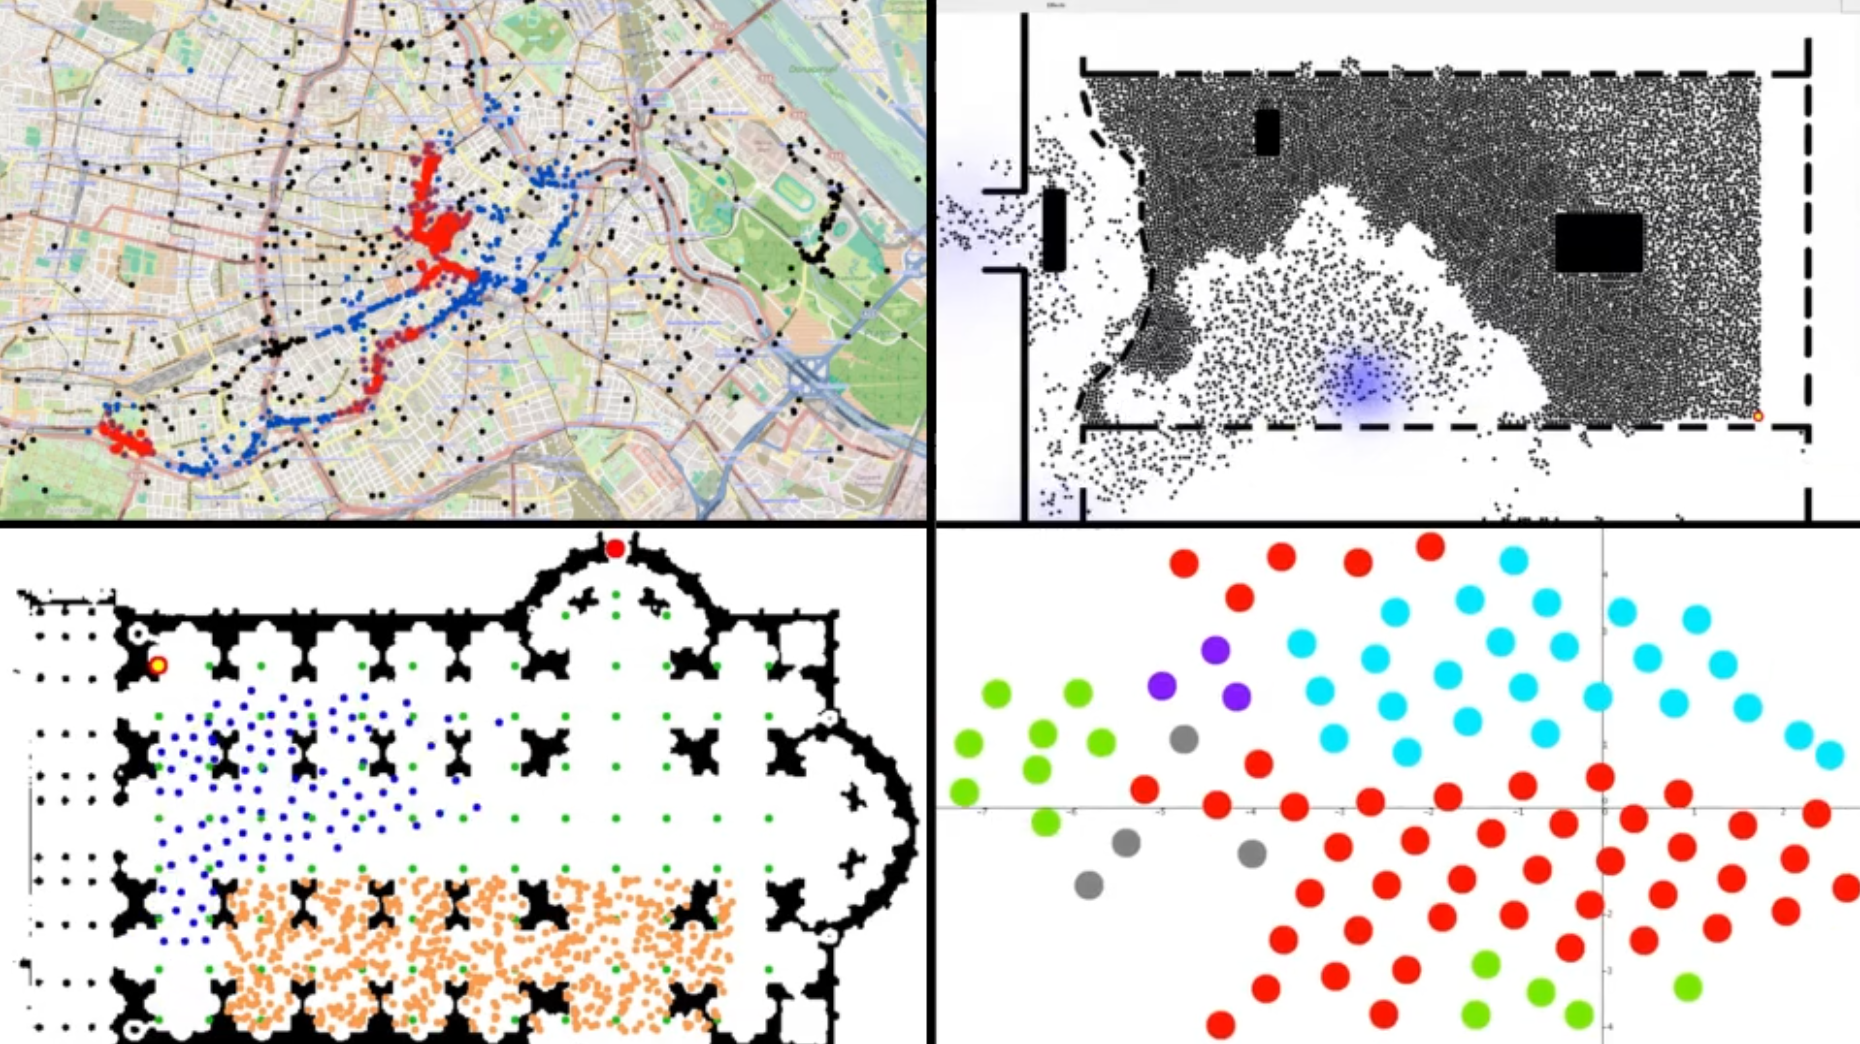
\includegraphics[width=0.5\textwidth]{img/alchemist-recap.png}
\end{center}
\end{frame}
\begin{frame}{Abstract model}
\centering
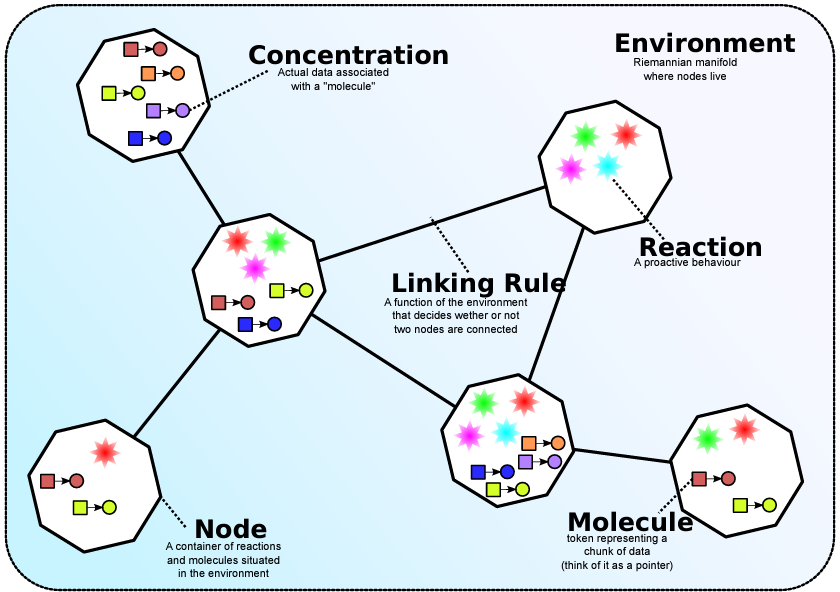
\includegraphics[width=0.8\textwidth]{img/abstract-model.png}
\end{frame}
\begin{frame}{Reactions}
\centering
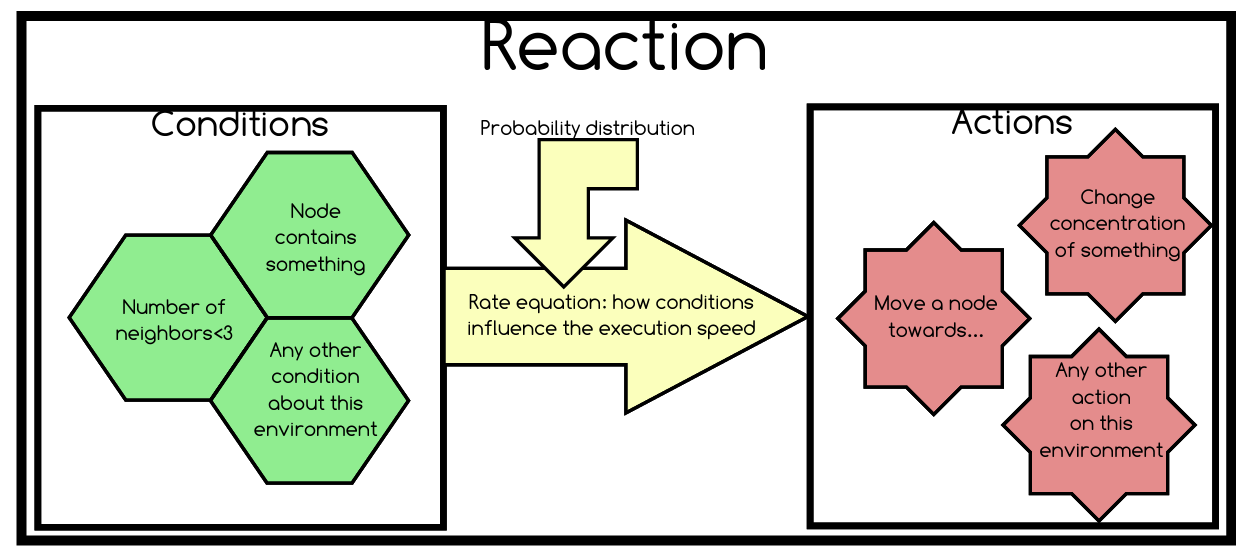
\includegraphics[width=0.8\textwidth]{img/reaction-model.png}
\end{frame}
\begin{frame}{Overall Architecture}
\centering
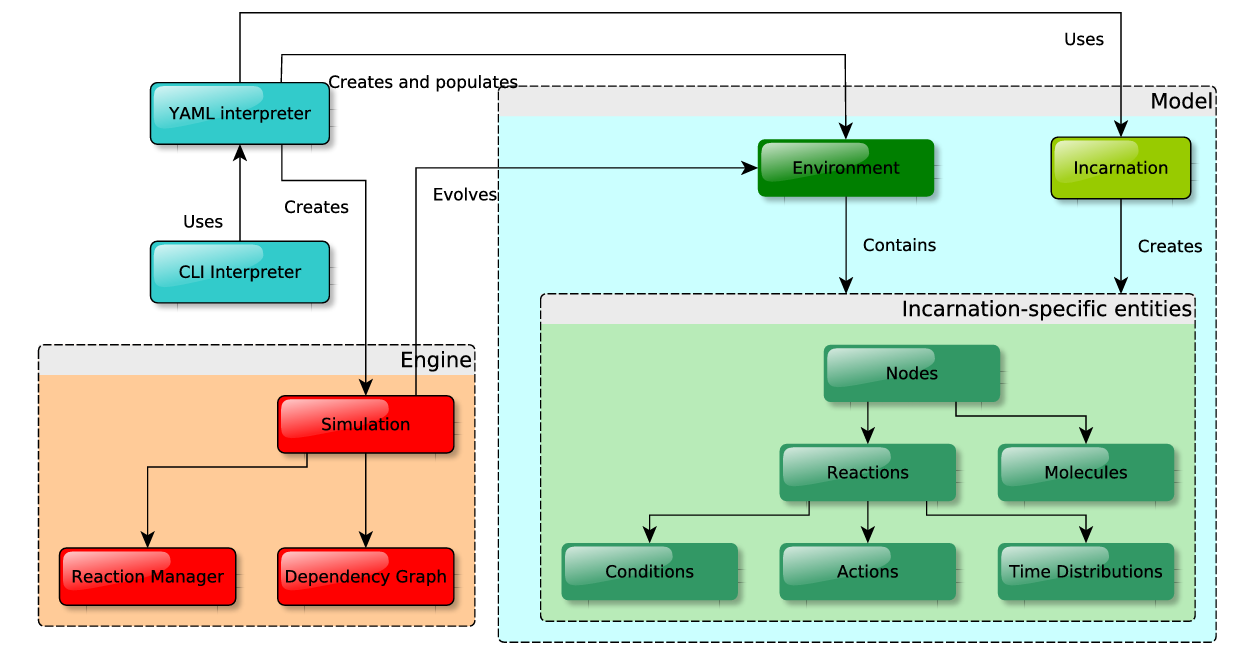
\includegraphics[width=0.8\textwidth]{img/alchemist-architecture.png}
\end{frame}
\begin{frame}{ScaFi Incarnation}
\begin{block}{Motivation}
	\begin{itemize}
		\item ScaFi has it own simulator \dots
		\item \dots but it is not as powerful as Alchemist, which:
		\begin{itemize}
			\item support GPS traces
			\item can simulate thousands of nodes
			\item can simulate different kinds of networks
			\item can simulate different mobility models
		\end{itemize}
	\end{itemize}
\end{block}
\begin{exampleblock}{ScaFi-Alchemist known uses}
	\begin{itemize}
		\item Swarm Robotics API: MacroSwarm\footnote[frame]{\fullcite{macroswarm}}
		\item Large-Scale smart cities simulations: FloodWatch\footnote[frame]{\fullcite{iee-floodwatch}}
		\item Crowd simulations
		\item \dots
	\end{itemize}
\end{exampleblock}
\end{frame}
\section{}

%===============================================================================

%/////////
\frame{\titlepage}
%/////////

%===============================================================================
\section*{\refname}
%===============================================================================

%%%%
\setbeamertemplate{page number in head/foot}{}
%/////////


%%%%%%%%%%%%%%%%%%%%%%%%%%%%%%%%%%%%%%%%%%%%%%%%%%%%%%%%%%%%%%%%%%%%%%%%%%%%%%%%
\end{document}
%%%%%%%%%%%%%%%%%%%%%%%%%%%%%%%%%%%%%%%%%%%%%%%%%%%%%%%%%%%%%%%%%%%%%%%%%%%%%%%%
